\documentclass[letterpaper,10pt]{article}

\usepackage{enumitem}
\usepackage{titling}
\usepackage{listings}
\usepackage{url}
\usepackage{hyperref}
\usepackage{setspace}
\usepackage{subfig}
\usepackage{sectsty}
\usepackage{pdfpages}
\usepackage{colortbl}
\usepackage{multirow}
\usepackage{multicol}
\usepackage{relsize}
\usepackage{amsmath}
\usepackage{wasysym}
\usepackage{fancyvrb}
\usepackage[yyyymmdd]{datetime}
\usepackage{amsmath,amssymb,amsthm,graphicx,xspace}
\usepackage[titlenotnumbered,noend,noline]{algorithm2e}
\usepackage[compact]{titlesec}
\usepackage{XCharter}
\usepackage[T1]{fontenc}
\usepackage[scaled]{beramono}
\usepackage[normalem]{ulem}
\usepackage{booktabs}
\usepackage{tikz}
\usetikzlibrary{arrows,automata,shapes,trees,matrix,chains,scopes,positioning,calc}
\tikzstyle{block} = [rectangle, draw, fill=blue!20,
text width=2.5em, text centered, rounded corners, minimum height=2em]
\tikzstyle{bw} = [rectangle, draw, fill=blue!20,
text width=4em, text centered, rounded corners, minimum height=2em]

\definecolor{namerow}{cmyk}{.40,.40,.40,.40}
\definecolor{namecol}{cmyk}{.40,.40,.40,.40}
\renewcommand{\dateseparator}{-}

\let\LaTeXtitle\title
\renewcommand{\title}[1]{\LaTeXtitle{\textsf{#1}}}

\lstset{basicstyle=\footnotesize\ttfamily,breaklines=true}

\newcommand{\handout}[5]{
	\noindent
	\begin{center}
		\framebox{
			\vbox{
				\hbox to 5.78in { {\bf ECE 350: Real-Time Operating Systems } \hfill #2 }
				\vspace{4mm}
				\hbox to 5.78in { {\Large \hfill #4  \hfill} }
				\vspace{2mm}
				\hbox to 5.78in { {\em #3 \hfill \today} }
			}
		}
	\end{center}
	\vspace*{4mm}
}

\newcommand{\lecture}[3]{\handout{#1}{#2}{#3}{Lecture#1}}
\newcommand{\tuple}[1]{\ensuremath{\left\langle #1 \right\rangle}\xspace}

\newcommand{\Rplus}{\protect\hspace{-.1em}\protect\raisebox{.35ex}{\smaller{\smaller\textbf{+}}}}
\newcommand{\Cpp}{\mbox{C\Rplus\Rplus}\xspace}


\addtolength{\oddsidemargin}{-1.000in}
\addtolength{\evensidemargin}{-0.500in}
\addtolength{\textwidth}{2.0in}
\addtolength{\topmargin}{-1.000in}
\addtolength{\textheight}{1.75in}
\addtolength{\parskip}{\baselineskip}
\setlength{\parindent}{0in}
\renewcommand{\baselinestretch}{1.5}
\newcommand{\term}{Spring 2023}
\newcommand{\termnumeric}{1235}

\singlespace


\begin{document}

\lecture{ 3 --- System Calls }{\term}{Jeff Zarnett}

\section*{System Calls: Remember, it's a Trap}

Operating systems run, as previously discussed, on interrupts. In addition to the interrupts that will be generated by hardware and devices (e.g., a keyboard signalling that the F1 key has been pressed), there are also interrupts generated in software. These are often referred to as a \textit{trap} (or, sometimes, an exception). The trap is usually generated either by an error like an invalid instruction or from a user program request.

If it is simply an error the operating system will decide how to deal with it, and in desktop/laptop OSes, the usual strategy is sending the exception to the program that caused it, and this is usually fatal to the offending program. Your programming experience will tell you that you can sometimes deal with an exception (perhaps through the language equivalent of the Java/C\# \texttt{try-catch-finally} syntax), but often an exception is unhandled and terminates the program.

The more interesting case is the intentional use of the trap: this is how a user program gets the operating system's attention. When a user program is running, the operating system is not; we might even say it is ``sleeping''. If the program running needs the operating system to do something, it needs to wake up the OS: interrupt its sleep. When the trap occurs, the interrupt handler (part of the OS) is going to run to deal with the request.

Already we saw the concept of user mode vs. supervisor mode instructions: some instructions are not available in user mode. Supervisor mode, also called kernel mode, allows all instructions and operations. Even something seemingly simple like reading from disk or writing to console output requires privileged instructions. These are common operations, but they involve the operating system every time.

Modern processors keep track of what mode they are in with the mode bit. This was not the case for some older processors and some current processors have more than two modes, but we will restrict ourselves to dual-mode operation with a mode bit. Thus we can see at a glance which mode the system is in. At boot up, the computer starts up in kernel mode as the operating system is started and loaded. User programs are always started in user mode. When a trap or interrupt occurs, and the operating system takes over, the mode bit is set to kernel mode; when it is finished the system goes back to user mode before the user program resumes~\cite{osc}.

Suppose a text editor wants to output data to a printer. Management of I/O devices like printers is the job of the OS, so to send the data, the text editor must ask the OS to step in, as in the diagram below:

\begin{center}
	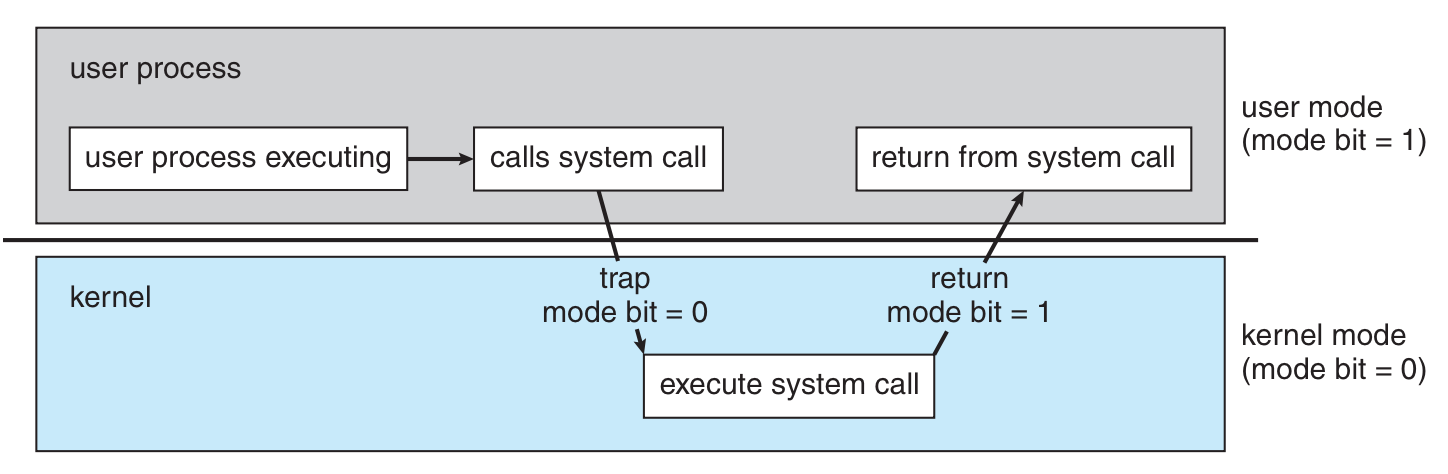
\includegraphics[width=0.75\textwidth]{images/trap.png}\\
	Transition from user to supervisor (kernel) mode~\cite{osc}.
\end{center}


So to print out the data, the program will prepare the data for printing. Then it calls the system call. You may think of this as being just like a normal function call, except it involves the operating system. This triggers the operating system (with a trap). The operating system responds and executes the system call and dispatches that data to the printer. When this job is done, operation goes back to user mode and the program returns from the system call.

\paragraph{Motivation for Dual Mode Operation.}

Why do we have user and supervisor modes, anyway? As Uncle Ben told Spiderman, ``with great power comes great responsibility''. Many of the reasons are the same as why we have user accounts and administrator accounts: we want to protect the system and its integrity against errant and malicious users.

An example: multiple programs might be trying to use the same I/O device at once. If Program~1 tries to read from disk, it will take time for that request to be serviced. During that time, if Program~2 wants to read from the same disk, the operating system will force Program~2 to wait its turn. Without the OS to enforce this, it would be up to the author(s) of Program~2 to check if the disk is currently in use and to wait patiently for it to become available. That may work if everybody plays nicely, but without someone to enforce the rules, sooner or later there will be a program that does something nasty, like cancel another program's read request and perform its read first.

This doesn't come for free, of course: there is a definite performance trade-off. Switching from user mode to kernel mode requires some instructions and some time. It would be faster if everything ran in kernel mode because we would spend no time switching. Despite this, the performance hit for the mode switch is judged worthwhile for the security and integrity benefits it provides.




\bibliographystyle{alphaurl}
\bibliography{350}


\end{document}